\section{Analysis}

\subsection{Fixed Points}

It is possible to calculate the fixed points of the discrete time mappings that govern the dynamics of the systems and compute their stability. By definition, these points will occur when $\mathbf{P}^{i+1}_L = \mathbf{P}^{i}_L$. In the case of the Open Model, these are trivial to compute. Consider \cref{eq:simple_update_rule}. There is an obvious fixed point at $\alpha = 1$. In this scenario, no matter what argument is presented, the listener will never be able to take that new information into account and will never update its beliefs, giving us a fixed point. To find others, we take $\alpha < 1$ to give a fixed point at $\mathbf{P}^i_L = \mathbf{A}^i_S$. This tells us that our second fixed point will occur when the speaker and the listener have identical probability distributions. To verify the stability of these, we compute the derivative of \cref{eq:simple_update_rule}. This yields

\begin{equation}
    \mathbf{P}^i_L = \alpha \cdot \mathbf{I} .
\end{equation}

Computing the eigenvalues of this equation shows that they are all equivalent to $\alpha$. This implies that for our fixed points, $\alpha = 1$ is stable and $\mathbf{P}^i_L = \mathbf{A}^i_S$ is stable since we assume that $\alpha < 1$, so all the eigenvalues lie within the unit circle. In the case of $\alpha = 1$, the eigenvalues equal $1$, meaning that the system is \emph{not} asymptotically stable. These two facts a supported by simulation and show that, when $\alpha = 1$ nothing happens, and when $\alpha < 1 $ the agents arrive at the same probability distribution that is a function of their initialisation. 

Taking the same approach with the Bottom Up and Top Down models, we can compute their fixed points in a similar way. Using the amended update rule in \cref{eq:BU_update_rule}, we get

\begin{align*}
    \mathbf{P}_L = \alpha \cdot \mathbf{P}_L + (1 - \alpha) \cdot \frac{\mathbf{A} \odot \mathbf{P}_L}{\mathbf{A} \cdot \mathbf{P}_L}.
\end{align*}

As above, we find one fixed point at $\alpha = 1$. The others can only exist when

\begin{align*}
    \mathbf{P}_L = \frac{\mathbf{A} \odot \mathbf{P}_L}{\mathbf{A} \cdot \mathbf{P}_L}.
\end{align*}

This tells us a number of things. Firstly, one can intuit from $\mathbf{A} \odot \mathbf{P}_L$ that the assertion $\mathbf{A}$ must contain every state of the world for which the listeners $p_i \neq 0$. From that, it is possible to say that $\mathbf{A} \cdot \mathbf{P}_L = 1$ since $\mathbf{A}$ can be represented as a column vector of $1$'s and $0$'s. 

Under these conditions, we compute the stability of the fixed points as follows. 
\begin{align}
    f(\mathbf{P}_L) &= \alpha \cdot \mathbf{P}_L + (1 - \alpha) \cdot \frac{\mathbf{A} \odot \mathbf{P}_L}{\mathbf{A} \cdot \mathbf{P}_L}\\
    \frac{d f(\mathbf{P}_L)}{d \mathbf{P}_L} &= \alpha \cdot \mathbf{I} + (1 - \alpha) \cdot \frac{d \frac{\mathbf{A} \odot \mathbf{P}_L}{\mathbf{A} \cdot \mathbf{P}_L}}{d \mathbf{P}_L}\label{eq:BU_stability}
\end{align}

\todo[color=James]{I am not sure if this should be identity matrix or a vector of 1's}
Focusing on the final derivative in the expression, 

\begin{align*}
    \frac{d \frac{\mathbf{A} \odot \mathbf{P}_L}{\mathbf{A} \cdot \mathbf{P}_L}}{d \mathbf{P}_L} &= \mathbf{A} \odot \mathbf{P}_L \cdot \frac{d \frac{1}{\mathbf{A} \cdot \mathbf{P}_L}}{d \mathbf{P}_L} + \frac{1}{\mathbf{A} \cdot \mathbf{P}_L} \cdot \frac{d \mathbf{A} \odot \mathbf{P}_L}{d \mathbf{P}_L}  \\
    &= \mathbf{A} \odot \mathbf{P}_L \cdot - \frac{\mathbf{A}}{(\mathbf{A} \cdot \mathbf{P}_L)^2} + \frac{1}{\mathbf{A} \cdot \mathbf{P}_L} \cdot \mathbf{A} \\
    &= \frac{\mathbf{A}}{\mathbf{A} \cdot \mathbf{P}_L} \cdot \left(  \mathbf{A} - \frac{\mathbf{A} \odot \mathbf{P}_L}{\mathbf{A} \cdot \mathbf{P}_L}  \right)
\end{align*}



Substituting this into \cref{eq:BU_stability},

\begin{align*}
    \frac{d f(\mathbf{P}_L)}{d \mathbf{P}_L} &= \alpha \cdot \mathbf{1} + (1 - \alpha) \cdot  \frac{\mathbf{A}}{\mathbf{A} \cdot \mathbf{P}_L} \cdot \left(  \mathbf{A} - \frac{\mathbf{A} \odot \mathbf{P}_L}{\mathbf{A} \cdot \mathbf{P}_L}  \right) \\
\end{align*}

As in the first case, the fixed point $\alpha = 1$ has eigenvalues at $\alpha$, again making it stable, though not asymptotically. The second fixed point requires a little simplification. Evaluating this equation at the fixed point gives,

\begin{align*}
    \frac{d f(\mathbf{P}_L)}{d \mathbf{P}_L} &= \alpha \cdot \mathbf{1} + (1 - \alpha) \cdot \frac{\mathbf{A}}{\mathbf{A} \cdot \mathbf{P}_L} \cdot \left(  \mathbf{A} - \mathbf{P}_L  \right)\\
    &= \alpha \cdot \mathbf{1} + (1 - \alpha) \cdot \left( \frac{\mathbf{A} \cdot \mathbf{A}}{\mathbf{A} \cdot \mathbf{P}_L} - \mathbf{1} \right) \\
    &= (2\alpha -1) \cdot \mathbf{1}  + (1 - \alpha) \cdot \frac{\mathbf{A} \cdot \mathbf{A}}{\mathbf{A} \cdot \mathbf{P}_L} \\
    &= (2\alpha -1) \cdot \mathbf{1}  + (1 - \alpha) \cdot \mathbf{A} \cdot \mathbf{A} \\
    &= (2\alpha -1) \cdot \mathbf{1}  + (1 - \alpha) \cdot |\mathbf{A}| \\
\end{align*}



\subsection{Consensus}

To gain an insight into the dynamics of these systems, let us consider their entropy, as defined by \cref{eq:shannon_entropy}. This serves as a measure of the uncertainty in the system such that high values imply the absence of strong beliefs in the population, and values close to zero imply a level of certainty, though, importantly, not consensus. To illustrate this distinction, consider \cref{fig:eg_bary}. Clearly, there are some agents in the corners who happen to be initialised with some strong beliefs in some states of the world. These agents will have low entropy values, whereas those closer to the centre of the plot will have much higher values due to their uncertainty. 

\begin{figure}[H]
 \centering
  \begin{minipage}[ht]{0.45\textwidth}
    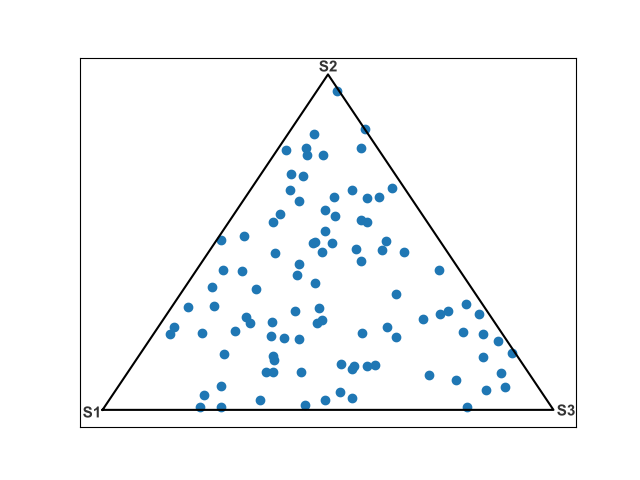
\includegraphics[width=\textwidth]{Images/Figures/OpenModel/open_model_BC_n_3_p_100_gullibility_0,3_runs_10.png}
 \end{minipage}
 \caption{ A Barycenter plot showing $100$ uniformly distributed agents in a world with 3 states.  }\label{fig:eg_bary}
\end{figure}

\Cref{fig:entropy_J_all} shows plots of entropy and J-divergence changing each iteration for each of the three models proposed. From the first plot it can be seen that the Open Model behaves very differently to the other two. In fact, the Open Model increases the entropy within a system, suggesting that the agents, on average, move away from the corners in \cref{fig:eg_bary}, decreasing their beliefs in some possible states of the world. The agents in this model essentially draw together, averaging their beliefs with every iteration that tends towards a uniform distribution. This is a function of the initial distribution though, not an inherent characteristic of the model. This increase in entropy suggests that this model is not a useful means of communication as it does not achieve reveal any strong sentiment in the cohort of agents, reducing their certainty in any possible state of the world to approximately uniform, and so shall not be extended.


\begin{figure}[H]
 \centering
  \begin{minipage}[ht]{0.49\textwidth}
    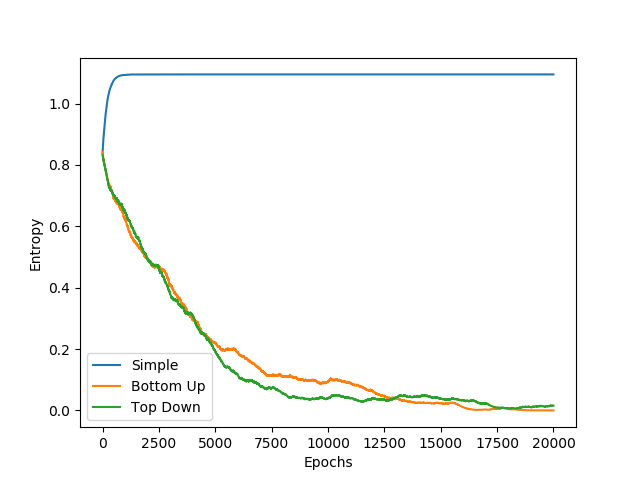
\includegraphics[width=\textwidth]{Images/Figures/Entropy/ALL_n_3_p_100_gamma_0,5_alpha_0,5.png}
 \end{minipage}
 \hfill
 \begin{minipage}[ht]{0.49\textwidth}
    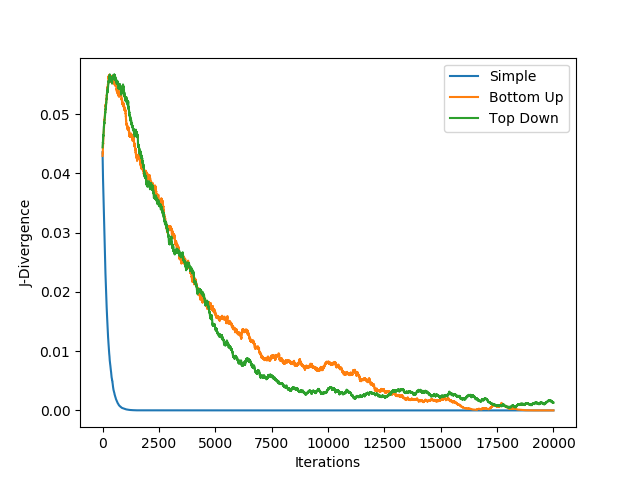
\includegraphics[width=\textwidth]{Images/Figures/All/ALL_n_3_p_100_gamma_0,5_alpha_0,5.png}
 \end{minipage}
 \caption{Two plots showing how entropy and J-divergence vary over time for the Open, Bottom Up and Top Down models/ These results were obtained using a value of $\alpha = 0.3$}\label{fig:entropy_J_all}
\end{figure}


This figure also shows that the Bottom Up and Top Down models behave very similarly. They both decrease the average entropy of the system to close to $0$ over time. These plots were created using $\gamma = 0.5$ to be as equivalent as possible. However, these plots serve solely to illustrate the general behaviour of the models. It can be seen that all models demonstrate some convergent behaviour over time, and two drive the agents toward high probability masses for at least $1$ state of the world. It is unclear from the entropy plot whether the agents have achieved consensus. 

The second plot serves to demonstrate consenting behaviour. The J-divergence is a symmetric version of KL-divergence, a distance metric well suited to probabilistic distances. This shows that the Open Model very rapidly reduces the distance between the agents, until it reaches $0$ after which there is no change. This fact, combined with the entropy plot show that agents in the simple model cluster together away from the edges of the plot in \cref{fig:eg_bary}. Conversely, the Bottom Up and Top Down models both converge to a single certain belief in one state of the world and then remain there. 



\subsection{Convergence}

In order to compare the behaviour of the two non-trivial models, consider their rate of convergence as given by Definition 2. Since they are not directly comparable for the same values of $\gamma$, the convergence time against $\gamma$ must be considered. \Cref{fig:convergence_none} shows three such plots. 

\begin{figure}[H]
 \centering
  \begin{subfigure}[ht]{0.45\textwidth}
    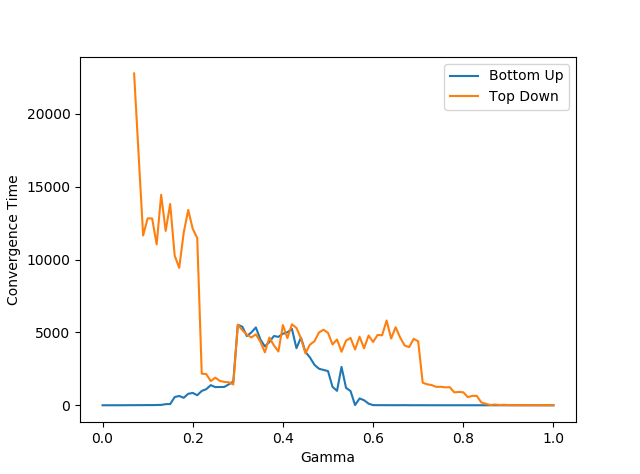
\includegraphics[width=\textwidth]{Images/Figures/All/Convergence_ALL_n_3_p_100_gamma_100_runs_20.png}
    \caption{Convergence}
 \end{subfigure}
 \hfill
 \begin{subfigure}[ht]{0.45\textwidth}
    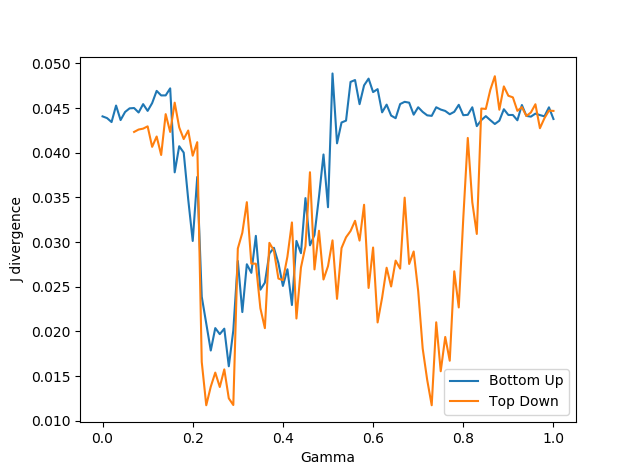
\includegraphics[width=\textwidth]{Images/Figures/All/J_Div_ALL_n_3_p_100_gamma_100_runs_20.png}
    \caption{J-Divergence}
 \end{subfigure}
 \hfill
 \begin{subfigure}[ht]{0.45\textwidth}
    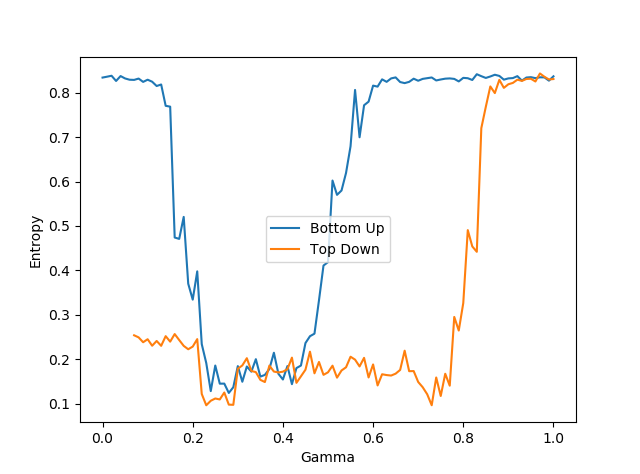
\includegraphics[width=\textwidth]{Images/Figures/All/Entropy_ALL_n_3_p_100_gamma_100_runs_20.png}
    \caption{Entropy}
 \end{subfigure}
 \caption{Three plots showing time to convergence, entropy and J-Divergence at convergence against a range of values for $\gamma$ for the Bottom Up and Top Down model. (\textit{$n=3, \alpha = 0.5, N = 100$ averaged over 20 runs. Convergence is defined as above using $t=3$, $\epsilon = 1 \times10^{-3}$})}\label{fig:convergence_none}
\end{figure}

It is apparent that, for both models, high values of $\gamma$ relate to very rapid convergence. This can be attributed to the fact that at values of $\gamma \approx 1$, it is impossible for either model to create a meaningful assertion; they are limited to asserting $\emptyset$ in the Bottom Up model and $\mathbf{W}$ for the Top Down which are both produce no reaction from the listening agent. This registers as very rapid convergence since the entropy does not change over time. 
In the the Bottom Up plots, one can observe that we get rapid convergence for values of $\gamma \geq \frac{1}{2}$. At this point, it becomes impossible for the speaker to assert anything other than a singleton, meaning that its arguments are guaranteed to be precise. This alone will increase the rate of convergence but another factor to consider is that as gamma increases, the only agents that can put forward any non-trivial argument are those who already hold extreme beliefs which high probability in one particular state. This accelerates the movement of the general population towards the region in which extremist speakers can speak until more and more of the population holds similarly strong beliefs and so more of them become able to assert something, perpetuating the effect. 

In the Bottom Up plots it is also possible to observe a sharp increase in convergence time shortly after $ \gamma = \frac{1}{n}$. As $\gamma$ increases above this point, it begins to create a region of probability space in which it is impossible for an agent to assert anything, making them purely passive, voiceless. For instance, if $\mathbf{P}_S =\{ 0.3, 0.3, 0.4\}$ and $\gamma = 0.5$, it is impossible for the speaker to assert anything. This will increase the convergence time as, if such an agent is picked, it is incapable of speaking, meanwhile, the agents that can speak are likely to be asserting slightly general statements so convergence is slow until $\gamma$ approaches $\frac{1}{2}$. 

The top down approach exhibits some different behaviour with slow convergence times for low values of gamma that appear to decrease for the most part. The slow convergence for low $\gamma$ is attributable oscillations in the dynamics of the system. At these low values, it becomes possible for the agents to assert states for which they have very little probability. This delays convergence by convincing listening agents to update their probability distributions in a way that increases the distance between the speaker and listener. 

The entropy and divergence plots reveal the state of the agents at time of convergence. High entropy implies that some agents do not have strong belief in one state, whereas the average pairwise J-Divergence suggests that they have failed to converge on a single state of the world. It can be seen that, for low values of gamma, we get a variety of different beliefs in the population, and that at least some of them are not certain in one state of the world alone. This is due to the lack of ability in the speaker to create non-zero arguments in the Bottom Up model, but as gamma increases there is a clear decrease in both entropy and J-divergence as both models find more flexibility in their expressions. As $\gamma$ increases, the Bottom Up model becomes less able to express its beliefs, and the extreme speakers are the only ones able to speak, decreasing the convergence times but, as the probability of the entropy changing very little over a number of iterations increases, so does the entropy and J-divergence. 

The Top Down model is shown to be more robust to changes in $\gamma$, with the majority of the agents holding strong beliefs at convergence, although they do not always agree on the strong belief as evidenced by the relatively high value of J-divergence. 

\subsection{Adaptions}

One key flaw in these models is that the agents are never able to ignore the speaker; they must take the assertion into account and react accordingly, even if it does not lead to a change of the listeners beliefs. This can be remedied by applying a threshold below which the listener agent will not attempt to update its beliefs. 

This is implemented by reversing the method by which the speaker creates its assertion. For example, in the Bottom Up model, the speaker includes every state of the world for which it has sufficient probability. In order to be more discerning, the listener will only update if every state in the speakers assertion is above $\gamma$ according to the listener, otherwise it will simply ignore the speaker. 

Similarly, the Top Down model requires that, from the listeners perspective, the speakers assertion has a probability above $\gamma$. The Open Model does not present any behaviour that encourages certainty in the population so it will no longer be considered



\begin{figure}[H]
 \centering
  \begin{subfigure}[ht]{0.45\textwidth}
    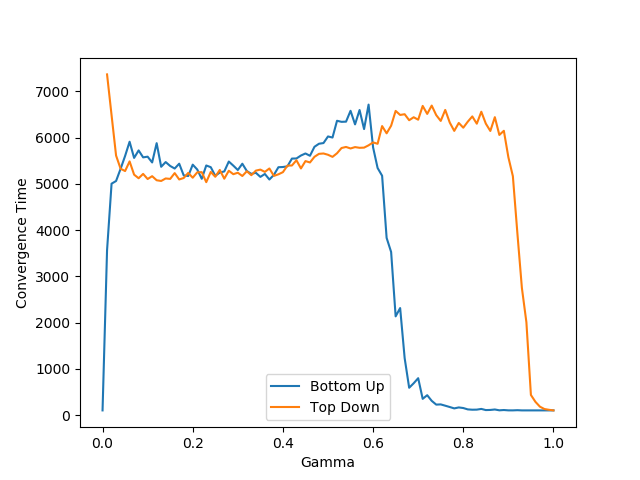
\includegraphics[width=\textwidth]{Images/Figures/All/Convergence_FIE_n_3_p_100_alpha_0,3_30_runs.png}
    \caption{Convergence}
 \end{subfigure}
 \hfill
 \begin{subfigure}[ht]{0.45\textwidth}
    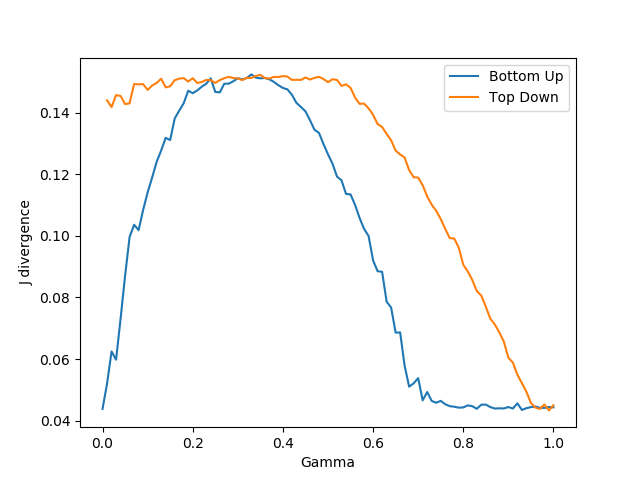
\includegraphics[width=\textwidth]{Images/Figures/All/J_Div_FIE_n_3_p_100_alpha_0,3_30_runs.png}
    \caption{J-Divergence}
 \end{subfigure}
 \hfill
 \begin{subfigure}[ht]{0.45\textwidth}
    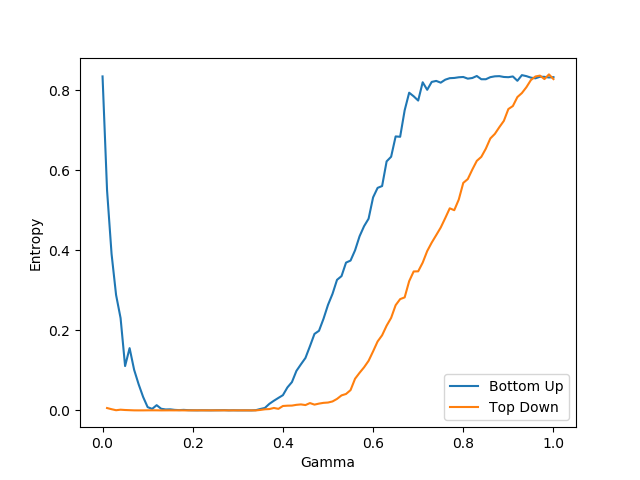
\includegraphics[width=\textwidth]{Images/Figures/All/Entropy_FIE_n_3_p_100_alpha_0,3_30_runs.png}
    \caption{Entropy}
 \end{subfigure}

 \caption{Three plots showing time to convergence, entropy and J-Divergence at convergence against a range of values for $\gamma$ for the Bottom Up and Top Down model, with discerning listeners. (\textit{$\alpha = 0.5, N = 100$ averaged over 20 runs. Convergence is defined as above using $t=100, \epsilon = 1\times10^{-5}$})}\label{fig:convergence_FIE}
\end{figure}


\Cref{fig:convergence_FIE} shows some similar traits to \cref{fig:convergence_none}, with rapid convergence at high values of $\gamma$. It should be noted that the condition for convergence was restricted severely to generate these plots. This is because, as listeners are now capable of disregarding speakers, the entropy in the system could remain constant for a small number of iterations, giving more of an inflection point than a steady state. 

As above, the rapid convergence for high $\gamma$ is due to few speakers being able to able to assert more than singleton arguments, however, now that the listeners are discerning, there is a chance for an uncertain listener to be able to ignore an opposing extreme speaker such that, while we may get convergence, we are unlikely to get consensus. In the entropy plot, the interval $0.1 < \gamma \leq 0.35 $ shows that the system reaches absolute certainty at steady state, however, for that same interval, the J-Divergence plot shows relatively high values. This suggests that the agents converge to the corners in a Barycenter plot, however do no agree on which corner to converge on. 

These plots show that for near zero values of $\gamma$, the Bottom Up approach produces rapid convergence, though not in such a way that the agents have decided anything, they simply maintain their probability distributions. The Top Down approach does not behave the same, instead, the agents converge on certain, disparate states of the world, although it does take $7,000$ iterations to do so. As gamma increases, both models tend to equivalence, producing almost identical results, with agents converging in $5,200$ iterations to opposing beliefs. As gamma increases further, both models lose their ability to evolve a population without uncertainty, suggesting that the agents converge to moderate beliefs, with moderation increasing with gamma until they converge almost immediately at their initial distribution, becoming ignorant of any new information a speaker might present as, when $\gamma = 1$, no matter how persuasive the speaker, the listener will not update. 


Another approach to handling disbelief in listening agents is to, instead of simply ignoring information they don't accept, grant them a more spiteful attitude. For instance, in the above case, if the listener disagrees with the assertion, it passively ignores it, but a more spiteful agent might instead take the complement of the assertion to be true, e.g. if the listener rejects an argument $\mathbf{A}$, it would then update using  

\begin{equation}
    \mathbf{P}^{i+1}_L = \alpha \cdot \mathbf{P}^{i}_L + (1 - \alpha) \cdot P(\cdot | \mathbf{A}^C). 
\end{equation}


\begin{figure}[H]
 \centering
  \begin{subfigure}[ht]{0.45\textwidth}
    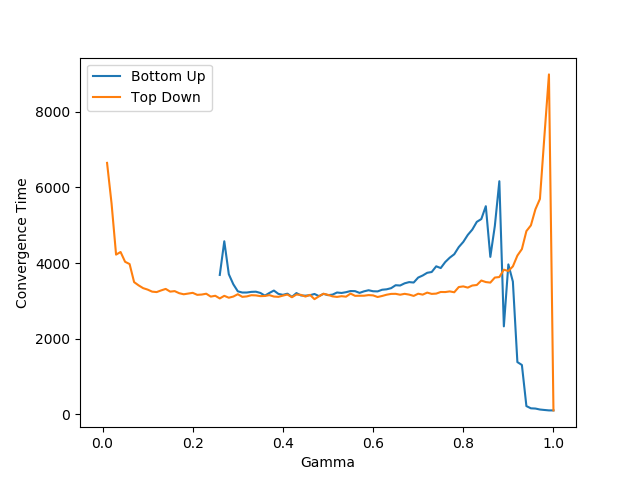
\includegraphics[width=\textwidth]{Images/Figures/All/Convergence_Spite_ALL_n_3_p_100_gamma_100_runs_20.png}
    \caption{Convergence}
 \end{subfigure}
 \hfill
 \begin{subfigure}[ht]{0.45\textwidth}
    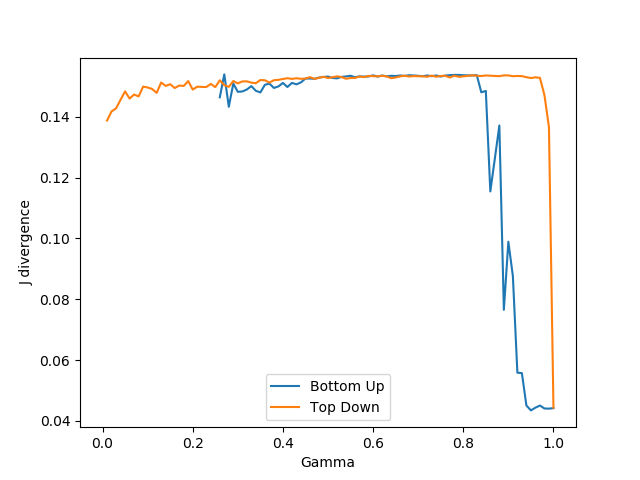
\includegraphics[width=\textwidth]{Images/Figures/All/J_Div_Spite_ALL_n_3_p_100_gamma_100_runs_20.png}
    \caption{J-Divergence}
 \end{subfigure}
 \hfill
 \begin{subfigure}[ht]{0.45\textwidth}
    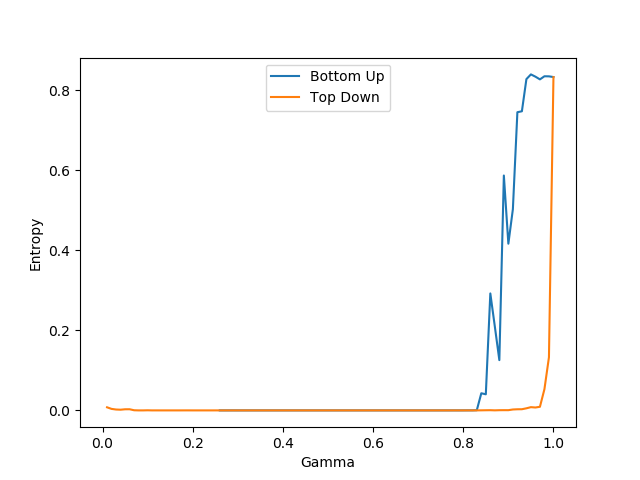
\includegraphics[width=\textwidth]{Images/Figures/All/Entropy_Spite_ALL_n_3_p_100_gamma_100_runs_20.png}
    \caption{Entropy}
 \end{subfigure}

 \caption{Three plots showing time to convergence, entropy and J-Divergence at convergence against a range of values for $\gamma$ for the Bottom Up and Top Down model, with discerning listeners. (\textit{$\alpha = 0.5, N = 100$ averaged over 20 runs. Convergence is defined as above using $t=100, \epsilon = 1\times10^{-5}$})}\label{fig:convergence_FIE}
\end{figure}

This more immature behaviour produces a drastic change in overall dynamics. The mechanism for both models to decide to ignore the speaker is the same as above. For high values of $\gamma$, the system again changes very little as the restrictions placed on both the speaker and the listener restrict the information that can be output or updated on so much that the system changes very little. For low values of $\gamma$, the Bottom Up model fails to converge at all. This is likely to occur when a speaker asserts a single state of the world, and the listener disagrees with it, instead updating on the complement, which cannot bring the listener to arrive at certainty in any single state of the world, provided $n>2$. The Top Down approach, however, produces convergence to certainty across a wide range of values for $\gamma$, although no consensus as the agents have high J-Divergence at steady state. 


The results presented above demonstrate that when agents openly express the exact nature of their beliefs, the population becomes uncertain. However, when they express arguments as certain states of the world, it becomes possible for the population as a whole to converge on a single state, provided the listener agents are indiscriminate in the information they use to update their beliefs. The Bottom Up and Top Down approaches achieve similar results, however the Bottom Up approach converges to a solution more rapidly than the Top Down. The Top Down model allows speakers to be more flexible with their assertions, allowing the majority of agents to reach certainty in a state at convergence. It is uncertain if either of these models outperforms the other, however it can be shown that the inclusion of discerning agents has a remarkable effect. When listeners ignore assertions that they do not already believe to have a degree of truth in it, they disregard it. This results in agents converging to distinct and certain probability distributions, sitting in opposing corners of a Barycenter plot, refusing to listen to any argument from another camp. 